\section{Implementation Issues and Performance Estimation}
\label{sec:issues}
The performance of a TC is commonly related to the ~\cite{biblio:tc_perf},
~\cite{biblio:tc_perf_2} following features: 

\begin{itemize}
    \item Timestamps accuracy 
    \item Correction factor stability
    \item Maximum update rate
    \item Rapid reconfiguration after topology changes
\end{itemize}

It applies to a WR TC as well.



WRS has been specially deceived to be compliant to most
common Ethernet standards (e.g. VLAN tags and Quality of Service) and fulfil demanding 
requirements in terms of upper-bound delivery, latency and fault tolerance. 
This features can be exploited to achieve remarkable performance as a TC.

\subsection{Time Stamping Accuracy}

In the chapter ~\ref{sec:wr}, the author resumes how WR accomplish
sub-nanoseconds synchronization and picoseconds jitter. It is based on the
characterization the asymmetries of the link a priory, and a clock lookback
technique. By doing this WR is able to  enhance the timestamps on ingress ports. 

The figure ~\ref{fig:time_stamp} shows that the Peer Delay timestamps between two 
adjacent nodes can be enhanced since the $pahse_{MM\_1}$ and $phase_{S\_1}$ to
the reference master clock signal are known. But it is not the case for $t_{2}$, 
this timestamp can be only enhanced using $phase_{S\_2}$ since the reference clock 
signal used in this link, is a synchronized clock to reference master clock signal 
(the same applies for $t_{4}$, in a E2E TC). The error introduced if the $t_{2}$ is 
enhanced using $phase_{S\_2}$ and not $phase_{S\_1}$ is:

x

x

x

x
Must be calculated!!!
x

x

x

\begin{figure*}[!t]
\centering
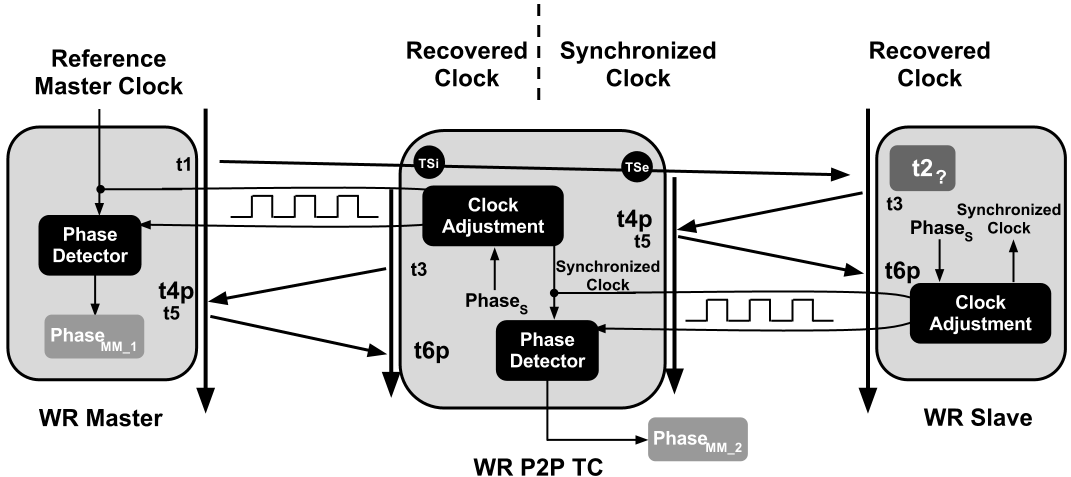
\includegraphics[scale=0.43]{fig/time_stamps_tc.png}
\caption{WR synchronization and P2P TC}
\label{fig:time_stamp}
\end{figure*}

\subsection{Correction Factor Stability and Maximum Update Rate}

Both, correction factor and  update rate, are features greatly influence
by the latency in the TC. As a result  synchronization could suffer
a degradation of the performance. An increment of the residence time in a TC normally is associated 
to increment of the traffic load handled by this TC. The authors of ~\cite{biblio:tc_perf} 
present the parameter \textit{Correction Factor Error} (CFE). It expresses the difference of the latency measured by a 
test equipment and the updated CF. The authors test TCs from different vendors
under high multicast load and compare the CFE result. 
The outcome of the test clarifies that switches with hardware treatment of the Sync messages 
maintain the CFE value low while the latency increases. Regarding
the WR TC, this is option that the  WRS enjoys already, hardware implementation 
of the timestamping unit, as well as hardware process forwarding of the Sync.

The \textit{Update Rate} (UR) for a two-step clock, is defined as the time between the transmission of a Sync
message from the master till the reception of the Follow Up message by the slave. 
High latencies, 10-30\% ~\cite{biblio:tc_perf} of the UR, can create 
instability in the slave. In addition, high latencies makes the TC no suitable for applications
demanding high UR. WRS is designed to provide low latency for time critical
information (e.g control accelerator information) using Cut-Through forwarding
schema and QoS \cite[vlan] in the output ports it is possible to queue the PTP
traffic in the second highest priority. By doing this the UR will be still high.

\FloatBarrier

\subsection{Reconfiguration after Topologies Changes}

The application of the timing system defines not only the requirements of accuracy, precision, 
but also the stability and continuation of the synchronization in the events
of(?) failure of TCs. The author doesn't (past/present??)
find references of this features for timing system based on PTP in the
literature. Nevertheless, the new timing system for GSI and CERN  have a demanding requirement
regarding the stability of the timing. 

TABLE

Both timing systems achieve resilience against network failures using redundant
topologies. Lowe layer protocols resolves the topology to a loop-free topologies. As
a result, the protocol sets port connected to cyclic paths to block/passive
state. In this case only the P2P TC still issues the synchronization between the
ports, and in both directions. As a result both clocks have the link delay
information. This offers the possibility of having immediately available the
link after change in the topology. It means that the reconfiguration time 
doesn't depend on TC anymore but in the  lower layer protocol. WRS has already a
proposals for implementing a transparent mechanism ~\cite{biblio:wrswitch} for
recovering from single points of failure in a redundant network.
